\chapter{Architettura dello strumento di testing}

In questo capitolo viene descritta l'architettura ...

\section{Modulo principale}

Il modulo \verb|main.pyw| costituisce il punto di ingresso dell'applicazione. La classe \verb|MainWindow| rappresenta la finestra principale, ed eredita le caratteristiche della classe \verb|QMainWindow|, definita nel framework PyQt. A differenza delle normali finestre di dialogo, la finestra principale deve essere unica all'interno dell'applicazione e prevede l'eventuale spazio per un barra dei menù, una barra di stato, un'area centrale in cui verranno posizionati i widget dell'interfaccia ed infine una serie di dock window, ossia finestre posizionabili e ridimensionabili dall'utente contenute nella finestra principale.

\begin{figure}[htbp]
\begin{center}
\includegraphics{images/mainwindowlayout.png}
\caption{Zone principali di una MainWindow}
\label{fig:pyqtMainWindow}
\end{center}
\end{figure}

Nel costruttore della classe \verb|MainWindow| sono inizializzate le strutture dati principali usate internamente per mantenere in memoria lo stato dell'applicazione e sono posizionati i componenti visuali. Si è cercato di mantenere la logica vera e propria dell'applicazione in moduli e classi esterni, per facilitare la gestione del codice. Di conseguenza gli unici due compiti delegati alla classe principale riguardano la costruzione dell'interfaccia grafica e il collegamento tra i segnali emessi dai widget in seguito all'interazione dell'utente e le funzioni di callback per la gestione degli eventi.

\subsection{Costruzione dell'interfaccia grafica}

Per la costruzione dell'interfaccia grafica esistono due metodologie possibili nell'ambito del framework Qt. La prima soluzione prevede la costruzione ed il posizionamento programmatico dei widget e dei layout, definendo cioè il modo in cui l'interfaccia sarà composta tramite chiamate nel codice agli appositi metodi delle classi che incapsulano i componenti visuali.

La seconda alternativa contempla invece l'uso di uno strumento visuale per questo compito, chiamato QtDesigner \footnote{\url{http://doc.trolltech.com/4.7/designer-manual.html}}. Utilizzando questo editor il programmatore può disegnare visivamente l'interfaccia grafica trascinando i widget da una barra direttamente sulla finestra principale e posizionarli a piacimento senza ricorrere al codice. E' inoltre possibile gestire visivamente anche le connessioni tra signal e slot dei widget in maniera rapida tramite un apposito editor. 

Le informazioni fornite a QtDesigner sono memorizzate successivamente in un file con estensione "ui", che deve essere poi tradotto in codice Python tramite un'apposita utility eseguibile da linea di comando, prima di poter essere utilizzato.

Sebbene l'uso di questo strumento possa risultare decisamente produttivo, specialmente per creare prototipi o per gestire più efficacemente interfacce grafiche complesse, si è scelto di non utilizzarlo e di costruire l'interfaccia dell'applicazione in maniera programmatica. La scelta è stata fatta soprattutto per motivi didattici, in quanto l'utilizzo di questo strumento visuale avrebbe potenzialmente nascosto la filosofia con la quale il framework Qt gestisce il posizionamento dei widget, ostacolando l'apprendimento e rendendo poi più difficili interventi manuali di modifica in un secondo momento. Inoltre, la costruzione programmatica fornisce sicuramente un grado di controllo maggiore per un'interfaccia non estremamente complicata come quella per l'applicazione da realizzare.

Il widget principale dell'interfaccia, che raggruppa al suo interno la maggioranza degli altri componenti, è un widget di tipo \verb|QSplitter|. Esso permette di posizionare al suo interno altri widget all'interno di due aree separate da una barra, ridimensionabili in larghezza o in altezza dall'utente. In questo caso, si è impostato l'orientamento in senso orizzontale, in modo da ospitare nella zona sinistra il componente del browser e nella zona destra l'elenco delle azioni e delle asserzioni registrate. In base alla risoluzione dello schermo, l'utente può ridimensionare lo spazio assegnato in orizzontale ad una delle due aree nel caso avesse la necessità di visualizzare più o meno informazioni sulla registrazione attuale.

Una volta istanziato il widget \verb|QSplitter| ed averne assegnato una referenza ad una proprietà della classe, esso è stato impostato come widget centrale della finestra tramite il metodo \verb|QWindow::setCentralWidget|. 

\lstinputlisting[float=h, caption=Definizione e posizionamento del widget principale ]{code/ui/main_splitter.py}

Di seguito sono creati e posizionati nelle due aree i widget delle tre aree principali, ossia la barra dell'indirizzo, il browser e la lista delle azioni registrate. Il codice per questo scopo è stato suddiviso in altrettanti metodi protetti della classe MainWindow, per una migliore leggibilità e mantenibilità. 

\subsubsection{La barra degli indirizzi}

Per realizzare la barra dell'indirizzo, attraverso la quale caricare una pagina nel browser sottostante, sono stati utilizzati un campo di testo semplice \verb|QLineEdit| e un bottone a pressione di tipo \verb|QPushButton|. Questi ultimi sono stati posizionati in orizzontale tramite un layout di tipo \verb|QHBoxLayout|, che gestisce in maniera automatica il posizionamento fluido del suo contenuto in base alle dimensioni del contenitore.

All'interno del metodo chiamato alla pressione del pulsante, è stato inserita della semplice logica per rendere compatibile il formato dell'url inserito dall'utente con quello atteso dal componente del browser. Poiché quest'ultimo internamente si aspetta un URL completo di protocollo, esso viene aggiunto in maniera automatica se non viene digitato nel campo di testo dall'utente, come avviene nei normali browser.

Siccome la visita di un determinato indirizzo viene considerata come un evento interessante ai fini della simulazione, se la funzione di registrazione è attiva questa azione viene aggiunta all'elenco di quelle compiute dall'utente. Usando questa caratteristica è possibile definire allo stesso modo il punto di partenza di un test: basterà infatti attivare la registrazione, inserire l'indirizzo da visitare e da lì cominciare con l'interazione.

\subsubsection{Il browser}

Il widget di tipo \verb|QWebView|, che visualizza effettivamente il contenuto delle pagine web, non viene istanziato e gestito direttamente dal modulo principale, come avviene per tutti gli altri widget. Si è infatti scelto di incapsularne le funzionalità all'interno del modulo \verb|simulator|, descritto in seguito nel dettaglio. Tutta la parte relativa alla simulazione e all'interazione con l'applicazione web viene implementata attraverso i metodi della classe \verb|QWebPage| e \verb|QWebView|, pertanto dall'esterno il modulo \verb|simulator| viene visto come un oggetto opaco. 

Come si è visto però il posizionamento dei widget nell'interfaccia è responsabilità esclusivamente della classe \verb|MainWindow|. Per questo motivo, da essa è possibile ottenere un riferimento al componente del browser attraverso il metodo \verb|simulator::getWidget()|.

Al di sotto del browser sono state posizionate una label per mostrare lo stato di caricamento delle pagine da visualizzare ed una per mostrare all'utente il selettore CSS selezionato tramite l'apposito strumento. Queste informazioni sono gestire dal modulo simulator, e per poterle raggiungere dall'esterno si è sfruttato il sistema di gestione degli eventi offerto da Qt. Grazie ad esso, la classe \verb|Simulator| definisce ed emette svariati segnali personalizzati, ai quali sono connessi gli slot definiti nella classe \verb|MainWindow|. Quest'ultima viene quindi notificata quando il simulatore esegue azioni di interesse per l'interfaccia grafica.

\lstinputlisting[float=h, caption={Comunicazione ad eventi tra MainWindow e Simulator}, label=code:loadingLabel ]{code/ui/loading_label.py}

Nel codice del listato ~\ref{code:loadingLabel} vengono connessi i segnali emessi dalla classe Simulator con i metodi di callback della classe MainWindow. In particolare, in corrispondenza dell'evento di inizio caricamento di una pagina, viene mostrata nell'interfaccia la label che notifica all'utente questo stato di attesa, poiché questa operazione può richiedere un certo periodo di tempo, a seconda della velocità di connessione.  

Sempre in questo estratto di codice, si può osservare la sintassi utilizzata per ricevere segnali con parametri. In questo caso, il simulatore aggiunge all'evento di selezione di un elemento un parametro di tipo \verb|PyQt_PyObject|, contenente un'instanza della classe PickedData che incapsula le informazioni sulla selezione dell'utente. Questa particolare sintassi per il tipo del parametro da ricevere è dovuta alla conversione necessaria tra i tipi del framework Qt, definiti in C++, e i tipi del framework PyQt, definiti in Python. 

\subsubsection{La lista delle azioni}

La lista delle azioni è stata collocata nel pannello destro del widget QSplitter principale. Per realizzarla, si è scelto di utilizzare il componente \verb|QTreeView|, il quale visualizza i dati tenendo conto di una gerarchia ad albero tra gli elementi da mostrare. I livelli intermedi possono essere contratti ed espansi, in modo che l'utente possa scegliere di quali informazioni mostrare i dettagli. 

Se la modalità di registrazione è attiva, in questo spazio vengono mostrate le azioni compiute dall'utente all'interno della pagina web significative ai fini della simulazione, come il click sui link e la compilazione di campi testuali. In aggiunta, tra un'azione e l'altra è possibile inserire le assertion, ossia particolari condizioni che il simulatore deve verificare durante l'esecuzione del test. Quest'ultime sono di fatto equiparabili alle azioni compiute dall'utente, in quando automatizzano una parte dei controlli visivi da effettuare per accertarsi del corretto funzionamento. Per questo motivo, sono presentate nella stessa porzione di interfaccia delle azioni, nell'ordine cronologico in cui sono state definite.

Per implementare la vista ad albero si è ricorsi al pattern MVC proposto dal framework PyQt, pertanto è stato necessario definire una classe model apposita che funge da tramite tra la struttura dati interna, nella quale le azioni registrate sono memorizzate, e la view, che deve mostrare tali dati nell'interfaccia. Questa implementazione verrà descritta più nel dettaglio in seguito, all'interno del paragrafo dedicato al modulo \verb|actions|.

\lstinputlisting[float=h, caption={Costruzione della vista ad albero e connessione dei segnali}, label=code:setModel ]{code/ui/action_tree.py}

Come si può osservare in ~\ref{code:setModel}, attraverso il metodo \verb|setModel| della classe \verb|QTreeView| viene indicato al framework quale classe si intende adoperare come model per la vista istanziata.

Nelle righe successive vengono poi creati due pulsanti di tipo QToolButton e collegati i relativi eventi di click con i metodi che comunicano al simulatore di iniziare la riproduzione delle azioni correntemente memorizzate, oppure di cancellare le azioni evidenziate.

Per quest'ultimo scopo nel metodo \verb|_onRemoveActionClicked| è necessario accedere direttamente al model impostato per la vista ad albero, poiché è questa classe che si occupa di gestire i dati, secondo il pattern MVC. Le azioni non vengono infatti rimosse direttamente richiamando un metodo della classe QTreeView. Sarà invece il model che notificherà la view di un cambiamento avvenuto nei dati sottostanti e ciò provocherà un'aggiornamento delle informazioni mostrate nell'interfaccia. 

In questo modo è garantita la sincronia dei dati in memoria con quelli presentati a video, senza che l'applicazione possa trovarsi in uno stato inconsistente sotto questo aspetto.

\subsubsection{La barra degli strumenti}

Creare una tipica barra degli strumenti è relativamente semplice all'interno del framework Qt: è sufficiente infatti richiamare il metodo addToolBar della classe \verb|QMainWindow|, che come visto prevede già lo spazio per ospitarla. I vari pulsanti nella barra sono invece rappresentati da oggetti di tipo \verb|QAction|, ai quali viene assegnata un'icona. 

Gli oggetti QAction non sono semplici pulsanti, ma rappresentano le azioni principali eseguibili dall'applicazione. Tramite appositi metodi si definiscono vari attributi di queste azioni, tra cui ad esempio le combinazioni di tasti che le attivano. La classe QAction viene definita in Qt per uniformare e centralizzare la gestione di queste azioni, che normalmente è possibile compiere in maniere differenti. Spesso infatti azioni come l'apertura o il salvataggio di un file sono raggiungibili sia dalla barra degli strumenti, sia dal menù principale dell'applicazione. Siccome l'azione che l'utente si aspetta di eseguire è in effetti la stessa, è opportuno che dal lato del codice venga utilizzata la stessa entità, in modo da evitare una possibile duplicazione.

I file di immagine per le icone utilizzate nell'applicazione sono gestiti tramite un file esterno in formato XML, nel quale indicare le risorse impiegate con i percorsi ed i nomi dei file. Per ogni risorsa è anche possibile specificare un identificativo utilizzabile nell'applicazione per reperire il file in maniera più agevole e leggibile, senza specificarne il percorso fisico. Per poter usare questa lista di risorse, è necessario compilare il file XML in codice Python tramite l'utility \verb|pyrcc4| ed poi importarlo nell'applicazione come fosse un comune modulo in Python.

Siccome la creazione di un oggetto \verb|QAction| è un'operazione comune e richiede un discreto numero di linee di codice per assegnare l'icona, il testo di descrizione e la combinazione di tasti, è stato creato un metodo statico apposta nella classe \verb|Gui| del package \verb|Utilities|.

\section{Modulo simulator}

Il modulo \verb|Simulator| costituisce il cuore dell'applicazione, poiché raggruppa le classi utilizzate per interagire con l'applicazione web da testare. La classe \verb|Simulator| al suo interno sfrutta la tecnologia QWebKit e ne pilota l'interfaccia per gli scopi della simulazione. Dall'esterno quindi non è necessario interagire direttamente con il browser, poiché la classe Simulator ne astrae ed estende le funzionalità, introducendo i concetti di azione dell'utente, di asserzione e di simulazione.

Il componente QWebKit presenta un'architettura altamente modulare, che permette di riutilizzare singolarmente le diverse parti che lo compongono in maniera efficiente. Nello specifico, è la classe \verb|QWebPage| che gestisce il caricamento delle pagine, la cronologia degli indirizzi visitati, le strategie di memorizzazione dei cookies, ed altri aspetti di alto livello. Ogni QWebPage contiene almeno un oggetto di tipo \verb|QWebFrame|, che modella invece un frame definito tramite i tag HTML \verb|<frame>| o \verb|<iframe>|. Attraverso un \verb|QWebFrame| si può poi accedere alla rappresentazione in memoria del DOM, selezionando e modificando i nodi presenti, rappresentati a loro volta dalla classe \verb|QWebElement|. 

Grazie alla modularità delle due classi appena descritte, si può evitare l'overhead dovuto al rendering vero e proprio della pagina web se questo non è necessario ai fini dell'applicazione (ad esempio poiché è sufficiente accedere alle informazioni nel DOM). Per visualizzare sullo schermo la pagina web è infatti disponibile l'apposita classe \verb|QWebView|, che essendo discendente della classe |QWidget| viene trattata come un qualsiasi altro componente dell'interfaccia grafica.

\subsubsection{Iniezione di codice Javascript nelle pagine web}

Per i motivi descritti nel capitolo riguardante le tecnologie utilizzate, si è scelto di accedere al DOM della pagina e di intercettare gli eventi dovuti all'interazione con l'utente tramite la libreria jQuery. Tutto il codice realizzato in javascript deve quindi poter essere iniettato all'interno della pagina web che viene caricata dal simulatore, prima di poterne utilizzare le funzionalità. 

La classe \verb|QWebFrame| fornisce un metodo apposta per questo scopo, chiamato \verb|evaluateJavaScript|. Come indica il nome, esso accetta come parametro una stringa di testo contenente del codice javascript, che viene eseguito nel contesto del frame specficato. Il valore di ritorno del metodo corrisponde al valore restituito dall'esecuzione dell'ultima istruzione Javascript.

Nel caso dell'applicazione sviluppata, viene ipotizzato l'utilizzo del solo frame principale. Questo vincolo ha semplificato la fase di iniezione del codice nelle pagine web, senza però limitare nel complesso le funzionalità dello strumento. Inoltre oggi l'uso dei frame all'interno delle pagine web viene fortemente sconsigliato poiché ne danneggiano l'usabilità e l'accessiblità, tant'è che i tag relativi all'inserimento dei frame sono stati rimossi dalla nuova specifica per l'HTML5 \footnote{\url{http://www.w3.org/TR/html5-diff/\#absent-elements}}. 

All'interno del costruttore della classe Simulator vengono letti i file che contengono la libreria jQuery ed i componenti dell'applicazione sviluppati in Javascript, ossia il registratore degli eventi, il generatore dei selettori CSS e lo strumento per selezionare gli elementi della pagina web (\verb|Picker|). Il contenuto di questi file viene quindi iniettato in ogni pagina nel momento in cui il componente \verb|QWebPage| segnala che il caricamento della pagina è completata tramite l'apposito  \verb|signal|. 

Prima di iniettare effettivamente il codice Javascript, esso viene manipolato per evitare potenziali conflitti con il codice Javascript già presente nella pagina corrente. Per evitare conflitti tra i nomi delle variabili jQuery definisce il metodo \verb|noConflict| che consente di usare questa libreria insieme ad altre che utilizzano il nome di variabile \verb|$| come alias per l'oggetto principale (succede ad esempio nel caso del framework Mootools \footnote{\url{http://mootools.net}}). 

All'interno della classe Simulator viene perciò definito un alias speciale per la variabile di jQuery \verb|$|, che viene sostituito a questo simbolo in maniera automatica prima di eseguire il codice Javascript nel contesto della pagina web. Questo passaggio è dimostrato nell'estratto di codice ~\ref{code:jqueryNoConflict}:

\lstinputlisting[float=h, caption={Caricamento della libreria jQuery con modalità no-conflict}, label=code:jqueryNoConflict]{code/ui/jquery_no_conflict.py}

Un altro aspetto da tenere in considerazione per il corretto funzionamento del codice Javascript iniettato interessa le tempistiche con le quali esso si trova a dover interagire con il DOM della pagina. Se il codice si trova infatti ad accedere al DOM mentre la costruzione dell'albero da parte del browser non è ancora completata, potrebbero verificarsi comportamenti inattesi poiché gli ultimi elementi della pagina potrebbero non essere ancora effettivamente stati aggiunti alla rappresentazione in memoria del DOM. La manifestazione tipica di questo fenomeno consiste quindi nella mancata selezione di alcuni elementi, considerati inesistenti. 

Siccome l'istante in cui viene terminato il caricamento della pagina a livello di rete non coincide necessariamente con l'istante in cui la rappresentazione in memoria del DOM è stata completata, per superare il problema non si può fare affidamento semplicemente sul segnale \verb|loadFinished| emesso dalla classe \verb|QWebPage|. Fortunatamente, il framework jQuery fornisce una semplice soluzione alla questione grazie al metodo  \verb|$.ready()|. La funzione anonima passata a questo metodo, contenente il codice da eseguire, viene richiamata solamente quando il caricamento del DOM è stato completato.

Oltre che per caricare il codice delle librerie, questo meccanismo è stato utilizzato anche per realizzare una delle due strategia di simulazione, che viene descritta più dettagliatamente in seguito, nel paragrafo dedicato al package \verb|actions|. Per ora è sufficiente dire che le azioni dell'utente che sono state registrate, come il click su di un link, vengono rieseguite facendo eseguire all'interprete Javascript il codice apposito, che riproduce l'evento come se fosse stato generato dall'utente.

\subsubsection{Comunicazione tra Python e Javascript}

Come si è visto in precedenza, il framework PyQt fornisce anche un modo più sofisticato per interagire con il contesto web dall'applicazione in Python, che permette di utilizzare oggetti in Python in maniera trasparente anche all'interno del codice Javascript.

\subsection{Sincronizzazione tra richieste HTTP e flusso di simulazione}

Uno dei problemi principali che ci si è trovati ad affrontare durante lo sviluppo dello strumento per il testing è costituito dalla necessità di sincronizzare il flusso di esecuzione delle azioni simulate con i tempi di caricamento delle pagine web da parte di QWebKit. 

Sebbene sia stato appena descritto il metodo per attendere il completamento della rappresentazione del DOM prima di eseguire codice Javascript, esso non risolve il problema di stabilire la tempistica corretta con la quale far eseguire le azioni registrate al simulatore. E' infatti la parte di applicazione in Python che si occupa di pilotare il simulatore, stabilendo il momento in cui esso deve eseguire una determinata azione. Tale operazione deve essere iniziata però solamente quando la classe \verb|QWebPage| ha terminato il caricamento della pagina, poiché in caso contrario il codice Javascript da iniettare per eseguire materialmente la simulazione degli eventi e delle asserzioni avrebbe un comportamento non prevedibile. 

Per garantire la sincronizzazione temporale dei vari passi della simulazione, la classe \verb|Simulator| implementa il metodo \verb|wait_load|, mostrato nell'estratto ~\ref{code:waitLoad}.

\lstinputlisting[float=h, caption={Gestione della sincronia da parte del simulatore}, label=code:waitLoad]{code/simulator/wait_load.py} 

Per sospendere l'esecuzione della simulazione fino al completo caricamento della pagina corrente viene utilizzato un ciclo nel quale si controlla periodicamente il valore assunto della proprietà \verb|_load_status|. Il ciclo viene interrotto quando il valore assunto indica il termine della fase di caricamento, oppure allo scadere di un timeout, onde evitare che il tempo di attesa sia indefinito qualora si verifichino problemi. 

Il valore della variabile di stato \verb|_load_status| viene modificato in maniera asincrona dallo slot associato al segnale \verb|loadFinished()|, emesso dal componente del browser. Una volta ricevuto l'evento, la variabile di stato viene impostata con valore nullo, per indicare che non è in corso il caricamento di alcuna pagina.

Nel caso in cui il metodo di attesa venga invocato senza che sia effettivamente in corso un caricamento, il ciclo non viene eseguito.

La soluzione adottata non ha presentato particolari problemi di prestazioni pur implementando di fatto una forma di "busy form of waiting", poiché i tempi di attesa sono generalmente molto brevi e sono comunque controllati da un timeout. Una soluzione più elegante da questo punto di vista potrebbe contemplare l'utilizzo della programmazione concorrente mediante thread, che aggiungerebbe però un ulteriore livello di complessità all'applicazione senza aggiungere nulla però agli scopi finali.

L'effetto collaterale indesiderato consiste però nel fatto che, utilizzando il ciclo di attesa, l'interfaccia dell'applicazione smette di essere reattiva all'interazione con l'utente. Per superare questo ostacolo, si è fatto uso del metodo \verb|QCoreApplication.processEvents|, con il quale si impone manualmente al processo di processare gli eventi in coda in arrivo dal sistema operativo sottostante. Normalmente il loop degli eventi, tipico di ogni applicazione dotata di interfaccia, viene gestito internamente dal framework Qt, ma in questo caso è stato indispensabile interagirci direttamente.

Il metodo \verb|wait_load| viene invocato automaticamente quando viene simulata un'azione di click su di un elemento. Se il click non provoca il caricamento di una pagina o una richiesta asincrona, l'applicazione non si pone in stato di attesa. In questo modo il fase di registrazione non è necessario preoccuparsi di questo dettaglio tecnico.

\subsection{Simulazione e richieste AJAX}

La questione riguardante la sincronizzazione risulta ancora più delicata se considerano anche le richieste AJAX che possono essere eseguite dall'applicazione web. In questo caso, prima di simulare le azioni e le asserzioni successive si è costretti ad individuare una strategia per stabilire con certezza quando le eventuali richieste AJAX sono terminate, per poter poi proseguire con il flusso della simulazione. 

La maggiore complessità di questo problema rispetto al precedente risiede nella natura asincrona delle richieste AJAX. A differenza di quanto avviene per quest'ultime, il caricamento di una nuova pagina è un evento prevedibile durante il corso della simulazione, ed è pertanto gestibile in maniera efficace grazie al segnale \verb|loadFinished| emesso dalla classe \verb|QWebPage|. 

Poiché oramai la tecnologia AJAX trova impiego nella maggioranza delle applicazioni web recenti, è sembrato opportuno dare la possibilità di usare lo strumento sviluppato per il test di applicazioni che fanno uso di richieste asincrone, ricordando che tra gli obiettivi posti giocano un ruolo importante la semplicità d'uso e che l'utilizzatore per ipotesi può non avere competenze sulle tecnologie web utilizzate. 

A tale proposito si consideri questo semplice scenario d'uso: l'utente clicca su di un link e dietro le quinte l'applicazione web invia una richiesta AJAX al server. Il server risponde con un messaggio, ed il contenuto del DIV sottostante al link viene aggiornato con il messaggio ricevuto, senza che la pagina venga ricaricata. A questo punto si desidera definire un test che verifichi il corretto funzionamento dell'applicazione web in base a questo scenario. 

Affinché il test sia realizzabile, è necessario che il simulatore attenda il completamento della richiesta AJAX prima di eseguire l'asserzione definita dall'utente sul contenuto del messaggio visualizzato dopo il click sul link. Se ciò non avvenisse, il test fallirebbe solamente a causa delle tempistiche con cui viene effettuato.

Sono da tenere poi presenti le seguenti condizioni aggiuntive. In primo luogo, non è possibile prevedere a priori il tempo impiegato per completare la richiesta asincrona, poiché esso dipende da fattori esterni non controllabili, come il tempo di risposta del server, la dimensione della risposta e la congestione della rete. In aggiunta, differenti richieste AJAX possono essere originate in parallelo dalla stessa pagina, siccome normalmente l'utente può continuare ad interagire con l'interfaccia dell'applicazione web mentre questa attende il completamento di una precedente richiesta asincrona.

\begin{figure}[htbp]
\begin{center}
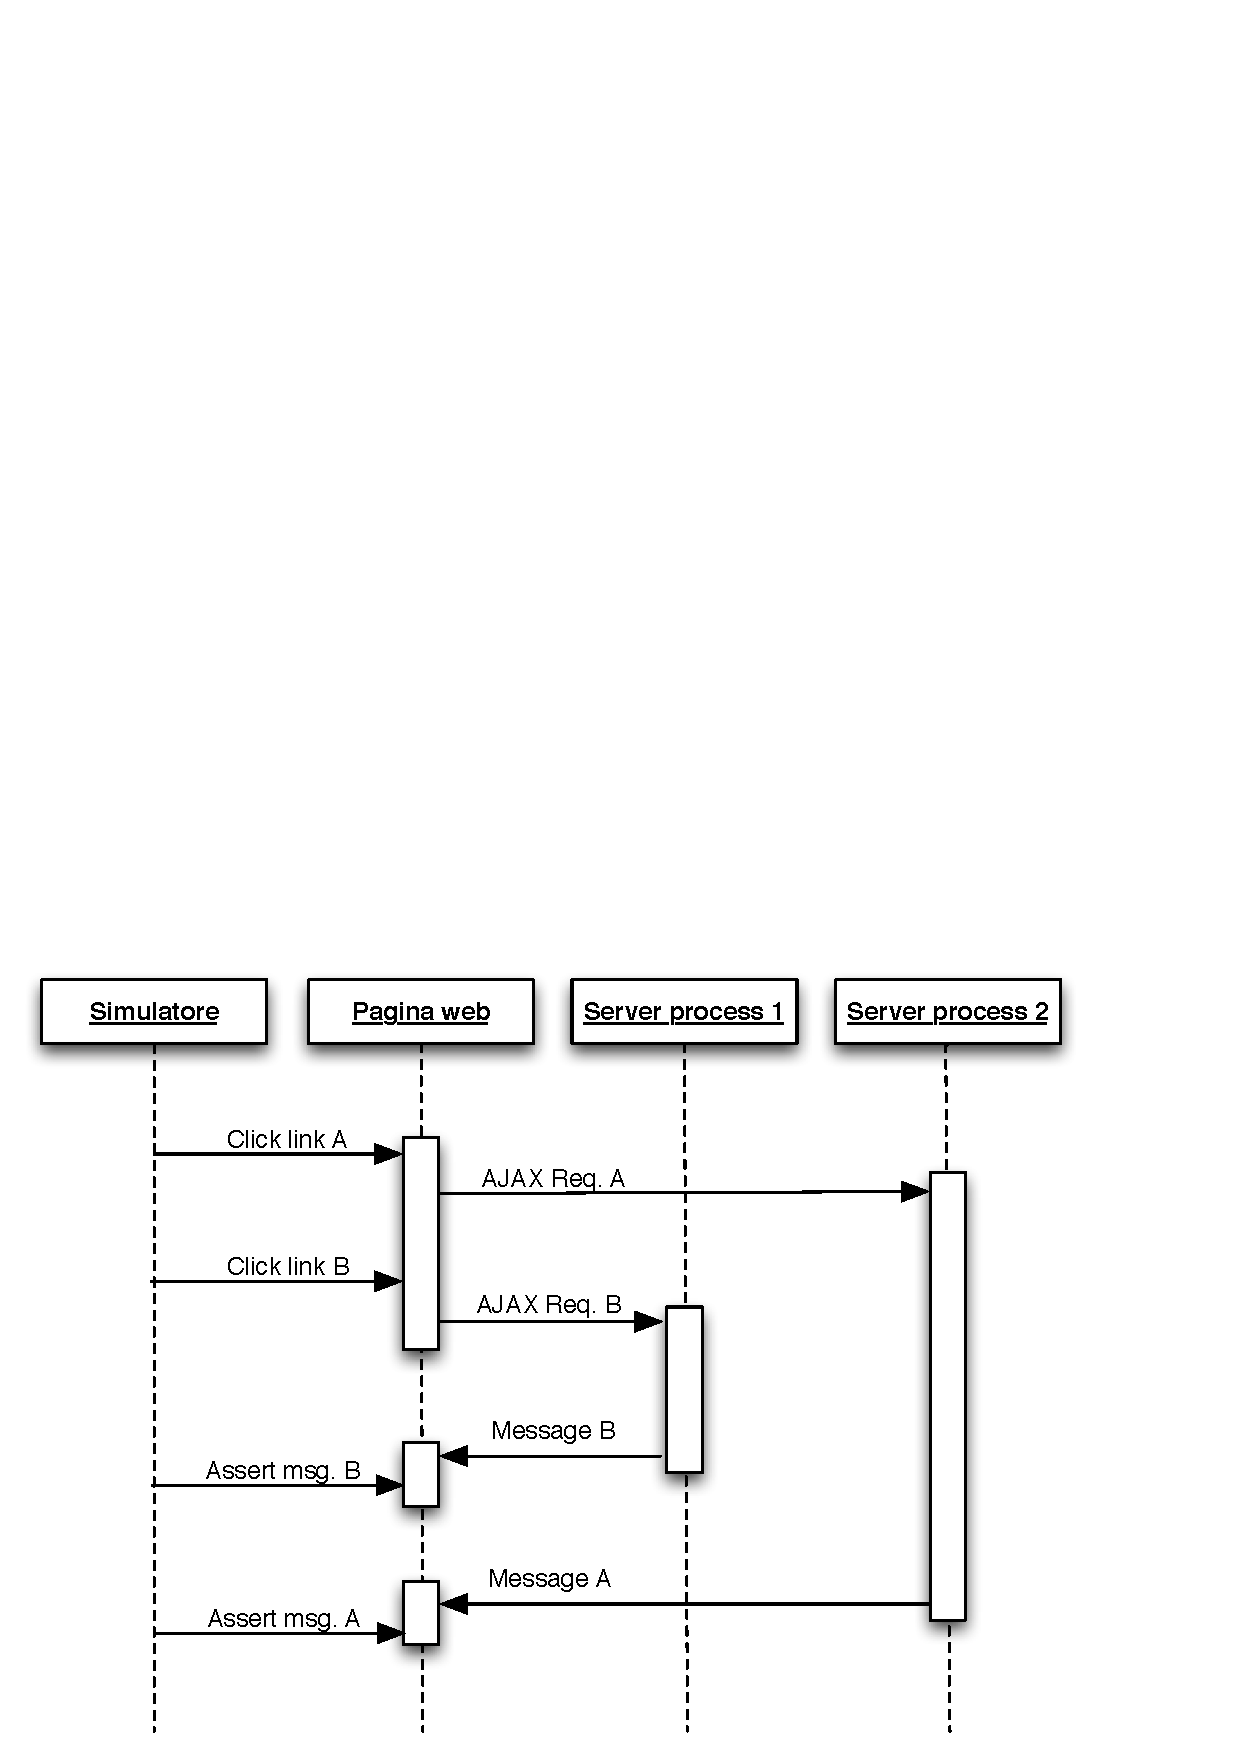
\includegraphics[width=\textwidth]{images/ajax_sync.png}
\caption{Sequence diagram per richieste AJAX parallele}
\label{fig:ajaxSequence}
\end{center}
\end{figure}

Nella figura ~\ref{fig:ajaxSequence} viene rappresentato un diagramma di sequenza che illustra la situazione descritta fino ad ora, con la corretta sequenza temporale in cui il simulatore dovrebbe effettuare le asserzioni nel caso in cui le richieste parallele ricevano risposte sfasate rispetto all'ordine di partenza.  

Per gestire le tempistiche in gioco per questo scenario non si può ricorrere al segnale utilizzato nel caso precedente, poiché questo non viene emesso dalla classe \verb|QWebPage| per le richieste asincrone generate una volta terminato il caricamento iniziale della pagina.

Per sapere quando una richiesta asincrona viene completata è stato necessario interagire ad un livello più basso del sistema, attraverso la classe \verb|QNetworkAccessManager|. Quest'ultima modella l'interazione a livello di rete del browser e permette di accedere ai dati delle singole richieste e risposte HTTP. Tra i segnali emessi, di particolare interesse è stato il segnale \verb|finished(QNetworkReply *)|, utilizzato per segnalare che è stata ricevuta una risposta ad una precedente richiesta e tale risposta viene passata come parametro al segnale. I dati di queste due entità sono incapsulati all'interno delle due classi \verb|QNetworkRequest| e \verb|QNetworkReply|.

Durante il caricamento della pagina il browser effettua diverse richieste HTTP attraverso il \verb|QNetworkAccessManager|, ad esempio per ricevere le immagini o altre risorse esterne alla pagina. Si è rivelato quindi necessario trovare un modo per distinguere le richieste AJAX dalle altre, che non richiedono un trattamento particolare. Per fare ciò si è scelto di analizzare gli header HTTP della richiesta, cercando come indicatori la presenza ed il valore del campo \verb|X-Requested-With|.

L'utilizzo di questo header particolare non è indicato nelle specifiche del W3C per quando riguarda le richieste di tipo XMLHttpRequest \footnote{\url{http://www.w3.org/TR/XMLHttpRequest}}, tuttavia può essere considerato uno standard de facto poiché tutti i maggiori framework Javascript (jQuery, MooTools, Prototype, YUI ed altri) lo includono automaticamente nelle richieste AJAX effettuate tramite queste librerie. Rimane però escluso il caso in cui l'applicazione sotto esame utilizzi il metodo nativo del browser per le richieste asincrone, senza aggiungere l'header \verb|X-Requested-With|. Sebbene sia probabilmente possibile stabilire un sistema di identificazione più raffinato, tenendo conto anche di questo caso, si è scelto di non approfondire la ricerca in questo senso per scarso interesse ai fini pratici, poiché oramai la stragrande maggioranza delle applicazioni web di una certa rilevanza si appoggiano su uno di questi framework Javascript \footnote{\url{http://trends.builtwith.com/javascript}}.

\vspace{1cm}
\lstinputlisting[float=h, caption={Identificazione di una richiesta AJAX terminata}, label=code:ajax_sniffing]{code/simulator/ajax_sniffing.py}

Il procedimento appena descritto è mostrato nel listato ~\ref{code:ajax_sniffing}. Come si può osservare, dopo che una richiesta asincrona è stata completata viene aggiornato di conseguenza il valore della proprietà \verb|load_status|, campionato durante l'attesa dal simulatore all'interno del metodo \verb|wait_load|.

Nel caso di richiese AJAX in parallelo, siccome il simulatore ne attende in automatico il completamento, di fatto esse vengono eseguite in maniera serializzata durante la simulazione, anche se l'utente non ha atteso la risposta alla prima richiesta prima di effettuare la seconda. Questa serializzazione forzata risulta indispensabile per eseguire nell'ordine corretto le eventuali asserzioni definite durante il test, senza che il loro risultato dipenda da fattori esterni non riproducibili.

\begin{figure}[htbp]
\begin{center}
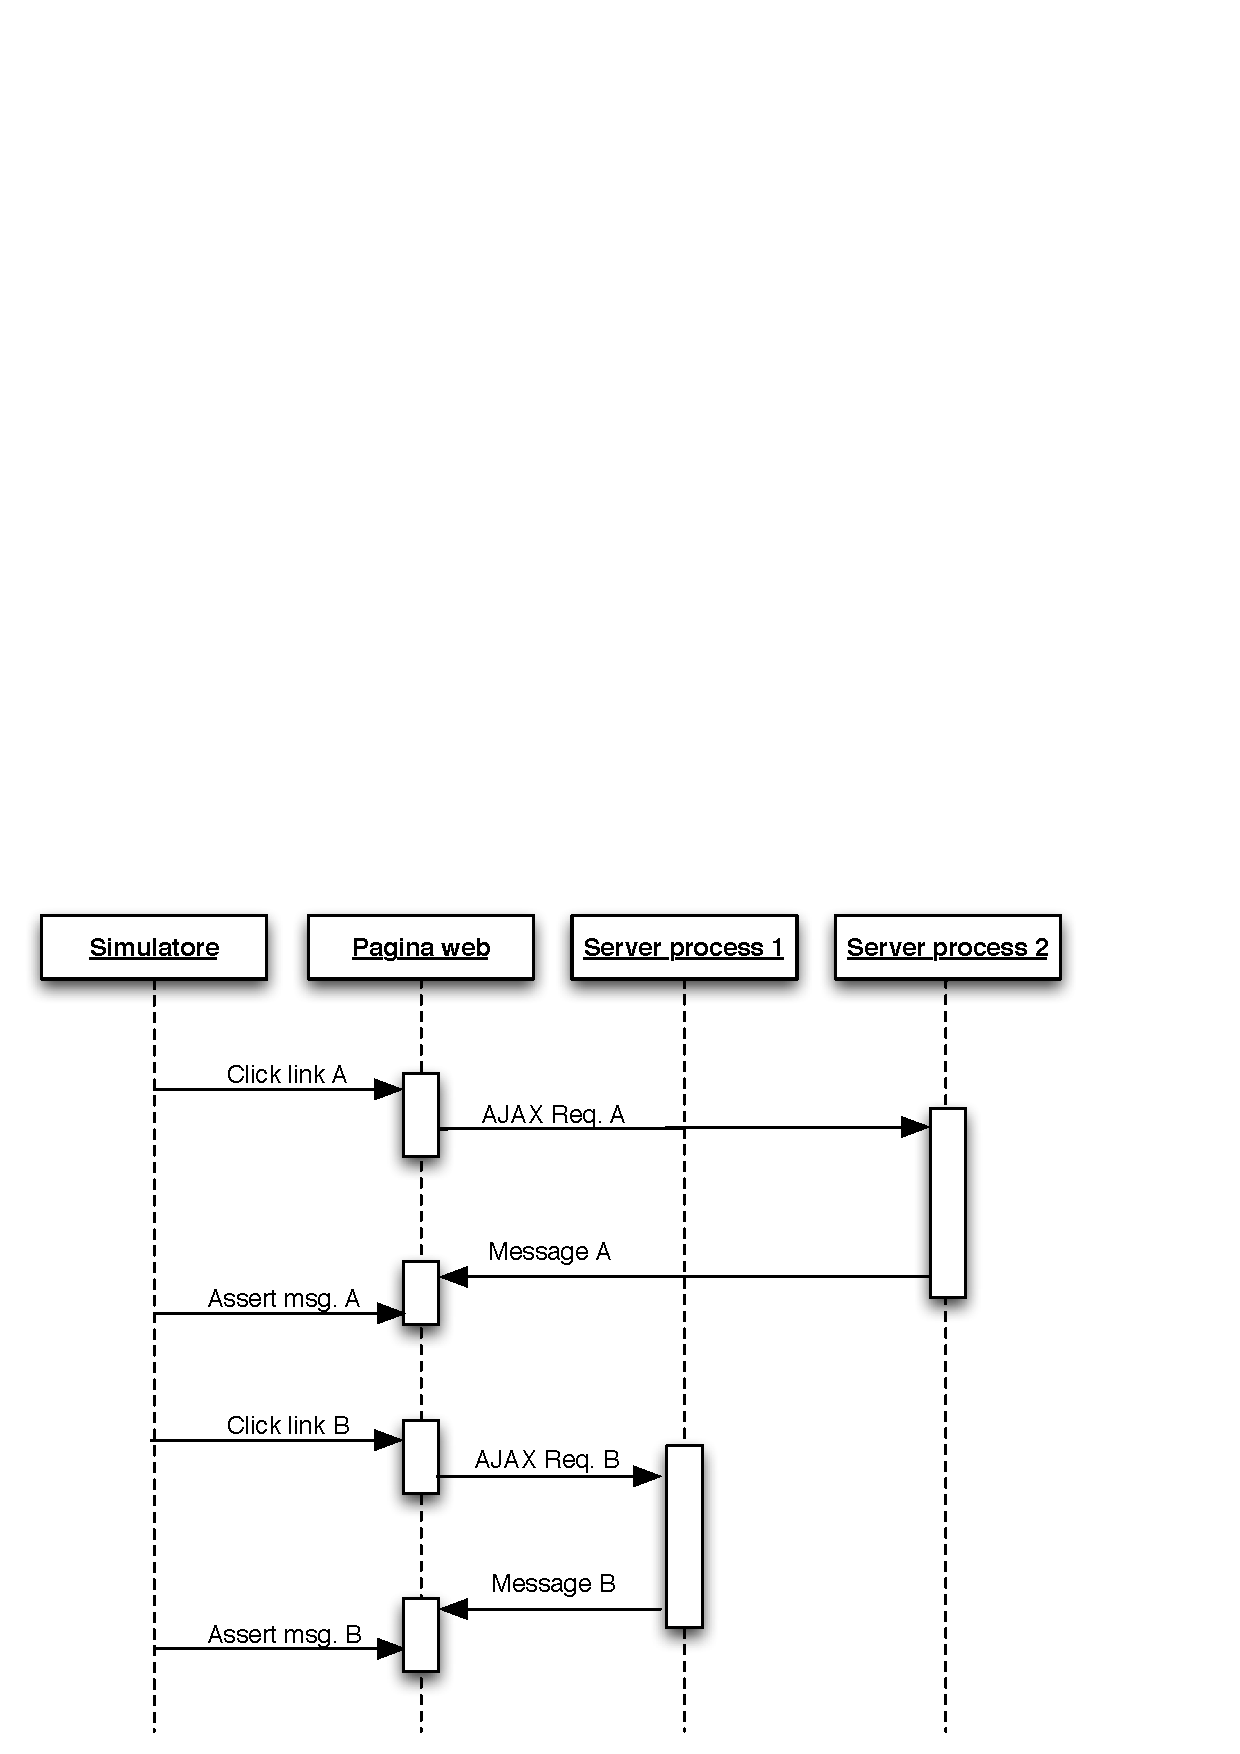
\includegraphics[width=\textwidth]{images/ajax_sync_for_simulation.png}
\caption{Sincronizzazione di richieste parallele durante la simulazione}
\label{fig:ajaxParallelSimulation}
\end{center}
\end{figure}

La figura ~\ref{fig:ajaxParallelSimulation} mostra come il simulatore gestisce uno scenario di test che contempli la presenza di richieste parallele, come quello indicato in figura ~\ref{fig:ajaxSequence}

\subsection{Riproduzione delle azioni}

Il controllo della riproduzione delle azioni registrate per il test viene delegato al metodo \verb|play| della classe \verb|Simulator|. Come parametro questo metodo riceve una lista di oggetti di classe \verb|Action|, itera sulla lista e su di  ognuna di esse invoca il metodo \verb|execute|. La logica vera e propria di esecuzione per le azioni e per le asserzioni è contenuta all'interno delle sottoclassi della classe \verb|Action|, che espongono l'implementazione specializzata del metodo statico \verb|execute|. Tale metodo viene richiamato passando come parametro un riferimento al simulatore, in modo che l'azione possa utilizzarlo per iniettare codice Javascript nella pagina o per effettuare altre operazioni necessarie.

Il metodo \verb|play| emette poi i segnali \verb|startSimulation| e \verb|endSimulation| rispettivamente all'inizio e alla fine della simulazione, i segnali \verb|startPlayAction|, \verb|endPlayAction| subito prima e subito dopo l'esecuzione di ogni singola azione. La classe della finestra principale intercetta questi eventi e aggiorna l'interfaccia grafica di conseguenza, evidenziando l'azione che si sta eseguendo in un dato momento nella vista ad albero.

\section{Modulo actions}

\subsection{Implementazione del Model nel paradigma MVD}

Come è stato descritto in precedenza, il framework Qt implementa il pattern MVD per gestire la visualizzazione dei dati nell'interfaccia grafica. La lista delle azioni viene mostrata all'utente attraverso una TreeView, cui è stato associato un model responsabile di manipolare l'accesso alla struttura dati principale, contenente le azioni registrate che compongono il test. 

La definizione di un model personalizzato ha consentito di avere un controllo maggiore sul modo in cui vengono mostrati i dati nella vista al albero, rispetto all'utilizzo del model generico già implementato all'interno del framework e pronto per essere abbinato alla TreeView nei casi più comuni. 

La struttura dati in cui sono memorizzate le azioni consiste in una lista semplice, una struttura dati già presente in Python attraverso il tipo List. Quando viene registrata una nuova azione, il model fornisce l'interfaccia per inserirla in questa lista, eseguendo poi una serie di operazioni non visibili dall'esterno. Una vista ad albero viene generalmente utilizzata per rappresentare una certa struttura gerarchica presente nei dati. Nel caso dell'applicazione realizzata, la gerarchia da visualizzare consiste in una lista di azioni, considerate come nodi padre, e per ciascuna di essere un'insieme di dettagli, visti come nodi figli della relativa azione. In questo modo l'utente potrà avvantaggiarsi della vista ad albero per visualizzare solo i dettagli di interesse, esplodendo i nodo padre.

Il model deve quindi occuparsi di costruire questa gerarchia, che di per sé non è presente nella struttura dati che memorizza le azioni. Essa infatti è una lista semplice e non un albero, poiché i dettagli di ogni azione sono in realtà memorizzati come proprietà degli oggetti di classe \verb|Action| contenuti nella lista stessa. Il model itera sulla lista delle azioni e da queste costruisce una struttura aggiuntiva ad albero che mappa ciò che la vista associata mostrerà effettivamente. Per i nodi di questo albero viene utilizzata la classe ausiliaria \verb|TreeItem|, che rappresenta un nodo di tipo principale oppure di dettaglio.

La classe \verb|TreeModel| si inserisce nell'architettura MVD del framework ereditando le funzionalità e l'interfaccia dalla classe \verb|QAbstractItemModel|. Per rispettare le convenzioni, essa deve reimplementare alcuni metodi definiti nella classe astratta. 

Nello specifico i metodi \verb|insertRow| e \verb|RemoveRow| si occupano di inserire e rimuovere gli oggetti dalla lista delle azioni e di notificare alla classe della vista il cambiamento dei dati, in modo da sincronizzarne la visualizzazione. Inoltre, quando si eseguono queste operazioni viene aggiornata di conseguenza anche la struttura ad albero interna.

 \lstinputlisting[float=h, caption={Costruzione della struttura dati ad albero interna al model}, label=code:buildTreeView]{code/model/convert_to_tree.py}

E' necessario inoltre reimplementare il metodo \verb|index|, poiché esso rende possibile alla classe \verb|TreeView| l'associazione tra i nodi della struttura ad albero nel model e gli elementi mostrati nella vista. In altre parole, la vista invoca il metodo \verb|index| per sapere quale dato mostrare nelle varie caselle del componente dell'interfaccia.

Una volta acquisito l'indice, la vista richiede al model il dato corrispondente. Per far ciò invoca il metodo \verb|data| del model, passando oltre all'indice anche un parametro indicante il "ruolo", ossia la modalità con cui i dati verranno usati. In base a questo parametro, la vista può richiedere i dati da utilizzare per mostrare il testo, per disegnare lo sfondo oppure un'icona, eccetera. Il model in base al ruolo richiesto fornisce se ne è in grado le informazioni richieste, accedendo alla struttura dati interna. 

Nel caso particolare dell'applicazione realizzata questo meccanismo viene utilizzato ad esempio per colorare in maniera differente lo sfondo di un elemento della vista al albero che rappresenta un asserzione, a seconda se essa abbia avuto esito positivo o negativo. E' importante notare che, siccome ci si trova ad operare all'interno del paradigma MVD, ogni cambiamento desiderato nelle viste deve essere rispecchiato da un cambiamento nei dati forniti dal model. La cronologia delle azioni che portano ad evidenziare di rosso un'asserzione fallita nella vista ad albero è la seguente:

\begin{enumerate}
\item La classe \verb|Simulator| nel \verb|play| invoca il metodo \verb|execute| sull'oggetto corrispondente all'asserzione corrente
\item L'azione effettua il controllo attraverso il simulatore. L'esito è negativo, la proprietà \verb|Assertion.passed| viene impostata a \verb|False|
\item Viene emesso il segnale \verb|dataChanged| dal model, la vista viene notificata di una modifica nei dati e deve ridisegnare l'elemento corrispondente all'indice ricevuto.
\item La classe \verb|TreeView| richiama il metodo \verb|data| del model indicando l'indice, con ruolo \verb|Qt.DisplayRole|, il model reperisce il dato tramite l'indice e restituisce la stringa da mostrare
\item La classe \verb|TreeView| richiama il metodo \verb|data| con ruolo \verb|Qt.BackgroundRole|, il model reperisce l'azione indicata dall'indice, verifica se è un'asserzione (istanza di \verb|Assertion|) e in tal caso restituisce un oggetto \verb|QBrush| con il quale la vista disegnerà lo sfondo della cella corrispondente. In caso contrario la vista userà le impostazioni standard per lo sfondo.
\end{enumerate}

\lstinputlisting[float=h, caption={Implementazione del metodo data per il model delle azioni}, label=code:modelData]{code/model/data_method.py}
 
\subsection{Salvataggio dei test in formato XML}

La classe \verb|TreeModel| si occupa anche di altre due operazioni che interessano i dati, ossia l'esportazione e l'importazione dei test in formato XML. Una volta registrata una sequenza di azioni, l'utente può scegliere di salvarla in un file XML su disco secondo il formato definito dall'applicazione, per poi poterla recuperare in un secondo momento.

Per il parsing e la generazione del formato XML con codifica UTF-8 è stato utilizzato il package \verb|xml.etree|, incluso nelle librerie standard fornite dal linguaggio Python, che con poche righe di codice ha consentito di eseguire tutte le operazioni necessarie.

Il metodo \verb|saveToXml| si occupa di creare la rappresentazione in memoria dell'albero XML partendo dalla lista di azioni memorizzate, per poi delegarne la serializzazione e la scrittura su file alle classi della libreria Python. La rappresentazione nel formato XML di ogni tipo di azione disponibile è gestita all'interno delle corrispondenti classi, che devono implementare il metodo \verb|toXML|. In questo modo si evita di accoppiare eccessivamente il codice del model con i dettagli interni di ogni azione.

Un esempio del formato XML utilizzato per rappresentare la sequenza di azioni è riportato nel listato ~\ref{code:xmlFormat} 

\lstinputlisting[float=h, language=xml, caption={Formato XML di un test case}, label=code:xmlFormat]{code/model/testcase.xml}

\subsubsection{Azioni ed asserzioni}

Le azioni eseguibili dal simulatore si classificano in due macrocategorie principali: azioni che simulano le operazioni dell'utente sull'interfaccia ed asserzioni che verificano alcuni aspetti circa il corretto funzionamento dell'applicazione.

Ognuna di queste azioni è stata modellata tramite un'apposita classe, contenente al suo interno la logica per l'esecuzione. Per facilitare l'implementazione di nuove azioni in aggiunta a quelle già presenti è stata impostata una gerarchia di classi, in modo da inserire le operazioni comuni nei livelli più alti della linea ereditaria. Tale struttura presenta le seguenti classi:

\begin{description}
\item[ ] La classe di base \verb|Action|, dalla quale ereditano tutte le altre azioni. Questa classe è astratta e definisce l'interfaccia che ogni sottoclasse deve implementare affinché possa essere utilizzata correttamente nell'applicazione.
I tre metodi indispensabili sono il metodo \verb|execute|, che deve contenere la logica per l'esecuzione dell'azione tramite l'istanza della classe \verb|Simulator| passata come parametro, il metodo \verb|fromXML|, che inizializza le proprietà della classe a partire dal nodo XML fornito in ingresso, ed infine il metodo \verb|toXML|, che si occupa di costruire il nodo dell'albero XML per la rappresentazione della classe. Questi ultimi due metodi sono utilizzati per importare ed esportare i test registrati.

\item[ ] La classe astratta \verb|UserAction|, che discende dalla classe \verb|Action| e modella un'interazione dell'utente con l'applicazione web sotto esame. Contiene il codice per gestire le proprietà comuni ad ognuna di esse.

\item[ ] La classe astratta \verb|AssertAction|, con funzioni analoghe alla precedente per le asserzioni.

\item[ ] Le classi che estendono \verb|UserAction|, raggruppate nel modulo \verb|actions.user_actions|, che definiscono una singola azione dell'utente.

\item[ ] Le classi che estendono \verb|AssertAction|, contenute nel modulo \verb|actions.assertions|, che rappresentato i vari tipi di asserzioni supportate dall'applicazione.
 
\end{description}

\begin{figure}[htbp]
\begin{center}
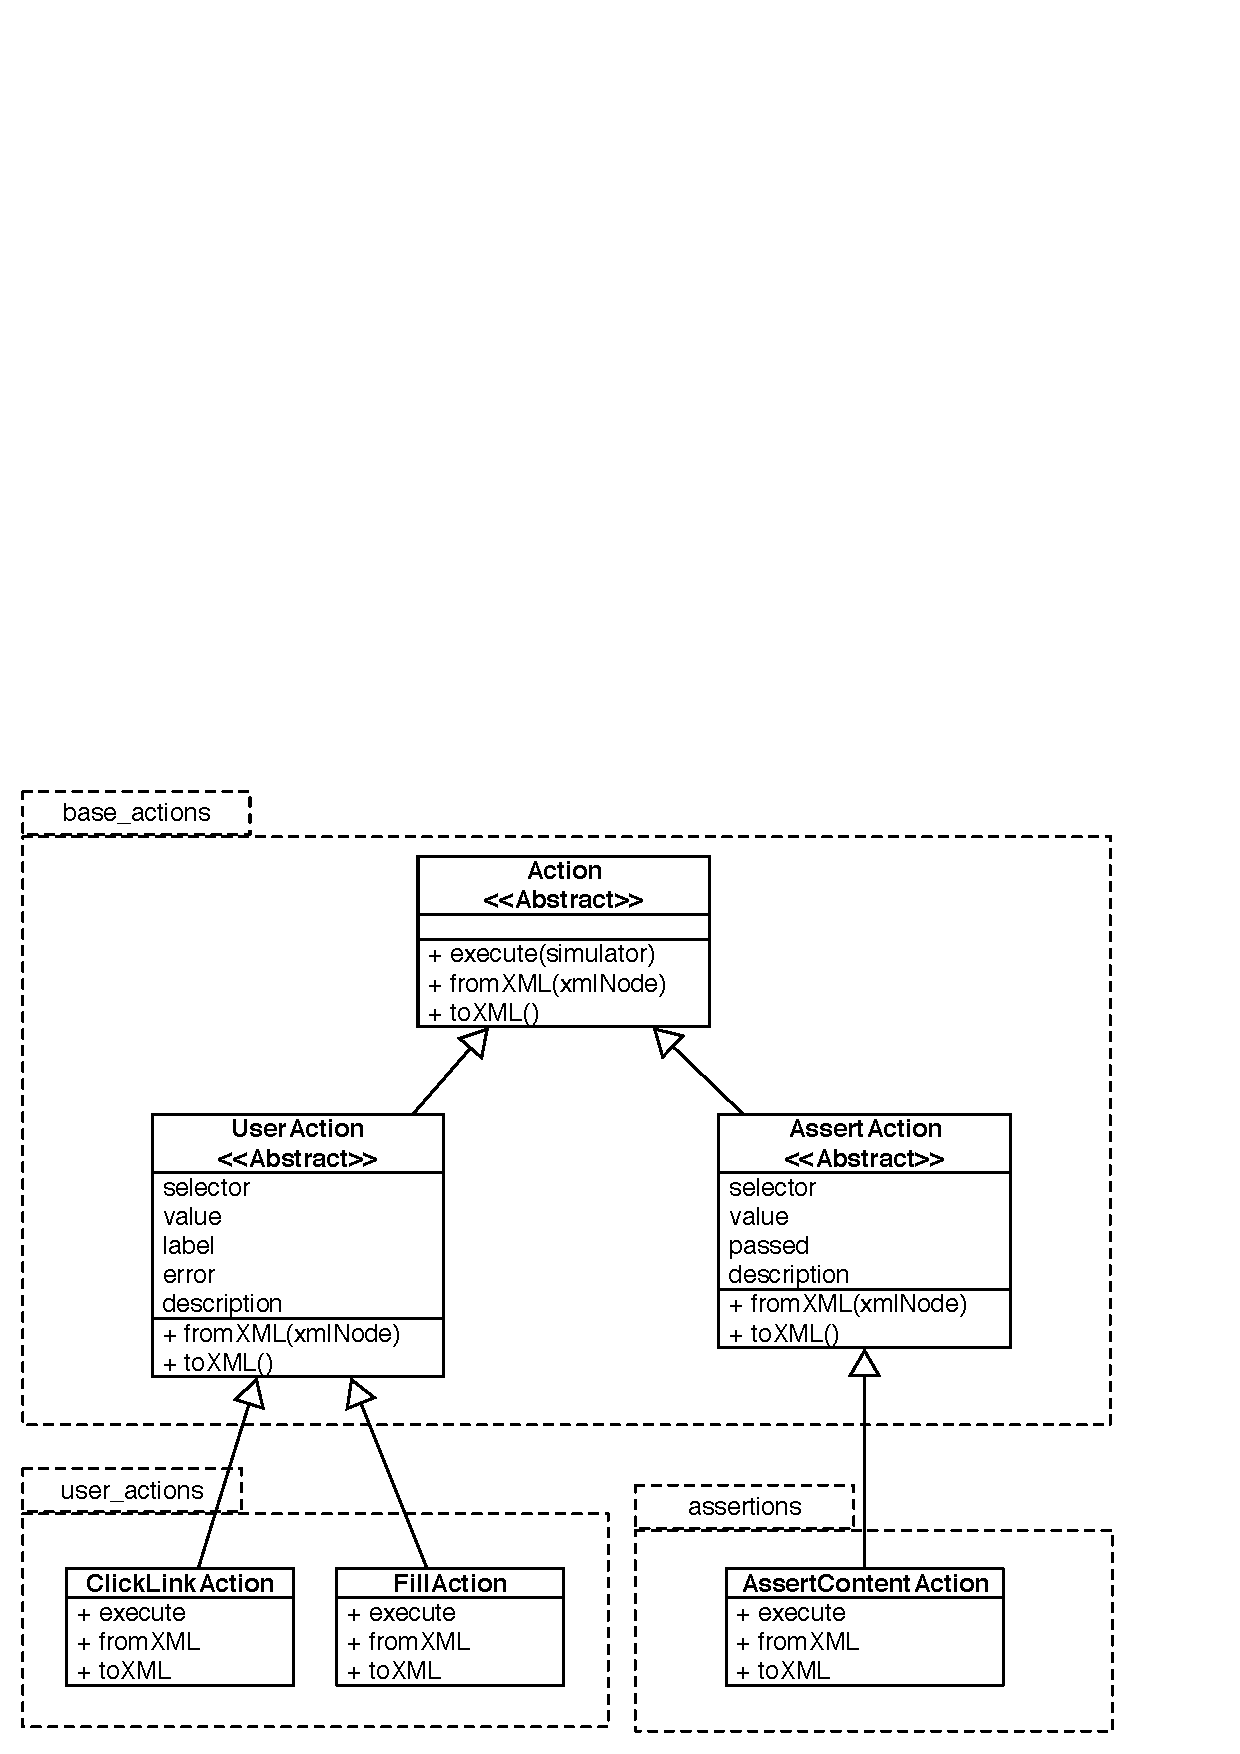
\includegraphics[width=\textwidth]{images/uml_actions.png}
\caption{UML diagram per il package delle azioni}
\label{fig:actionUML}
\end{center}
\end{figure}

Nel listato ~\ref{code:clickLinkAction} viene presentata a titolo esplicativo la classe \verb|ClickLinkAction|, che simula il click dell'utente su di un collegamento ipertestuale. Nel metodo \verb|execute| viene utilizzata l'istanza della classe \verb|Simulator| passata come parametro per eseguire il codice Javascript che simula effettivamente l'evento e per fermare il flusso di esecuzione dei test fino al completamento dell'eventuale richiesta HTTP generata dal click.

\lstinputlisting[float=h, language=Python, caption={Dettagli implementativi della classe ClickLinkAction}, label=code:clickLinkAction]{code/actions/click_link_action.py}

Aggiungere nuove azioni disponibili nell'applicazione in un secondo momento non richiede particolari modifiche al codice, oltre all'implementazione della relativa classe. Grazie al sistema di tipizzazione dinamica (duck typing) tipico del Python e di altri linguaggi non compilati, l'applicazione sarà in grado di utilizzare direttamente le funzionalità esposte dalla nuova classe.

\subsection{La registrazione delle azioni utente}

La cattura delle interazioni tra l'utente e la pagina web viene effettuata usando il meccanismo di gestione degli eventi del DOM. Utilizzando la libreria jQuery è possibile definire delle funzioni di callback, invocate quando un determinato evento raggiunge l'elemento specificato. 

\subsection{DOM event model}

Il motore WebKit utilizzato nel framework Qt adotta la specifica del W3C per il la gestione degli eventi nell'ambito del DOM \footnote{\url{http://www.w3.org/TR/DOM-Level-2-Events/events.html}}, pertanto si è fatto riferimento a queste direttive per identificare una strategia adatta alla cattura degli eventi generati dall'utente. 

In tale specifica vengono definiti le proprietà dell'evento, il modo in cui un evento si propaga nell'albero del DOM e la possibilità di registrare per un nodo dell'albero uno o più \verb|EventListener|, ossia una funzione da eseguire quando l'evento di tipo specificato raggiunge quell'elemento.

La propagazione degli eventi nel DOM viene divisa in due fasi distinte. Durante la prima fase, chiamata \emph{Event capture}, l'evento viene propagato in senso discendente nell'albero, dal nodo padre al nodo figlio, fino a raggiungere l'elemento specificato come "target" dell'evento. Le funzioni registrate come EventListener per questa fase possono così manipolare l'oggetto che rappresenta l'evento prima che esso raggiunga il nodo direttamente interessato. E' importante notare che solamente i nodi dell'albero che appartengono alla linea di discendenza del nodo target hanno la possibilità di interagire in questo processo di propagazione. Inoltre, gli EventListener vengono registrati esclusivamente in base alla tipologia dell'evento.

Dopo questa fase discendente, l'evento raggiunge il nodo target e ha inizio la fase di \emph{Event bubbling}, simmetrica alla precedente. L'evento infatti risale nella gerarchia dell'albero dal nodo di destinazione fino alla cima e vengono attivati tutti gli EventListener dei nodi interessati da questo percorso e definiti per questa fase, nell'ordine in cui sono stati registrati.

All'interno di un EventListener è inoltre possibile decidere di fermare la propagazione dell'evento oppure decidere di cancellarne l'azione normalmente associata, neutralizzandone di fatto l'effetto.

L'implementazione di WebKit fornisce quindi l'interfaccia Javascript necessaria per intercettare gli eventi nel DOM, tuttavia si è scelto di utilizzare la libreria jQuery poiché essa facilita la gestione degli eventi e offre funzionalità di livello più astratto rispetto all'implementazione nativa, che permettono di trascurare buona parte dei dettagli più difficili da trattare.

\subsection{Registrazione degli eventi}

Attraverso il metodo \verb|jQuery.bind| viene registrata una funzione di callback per il tipo di evento specificato come parametro. Grazie all'interfaccia fluente della libreria, questo metodo è invocabile direttamente su un insieme di oggetti del DOM selezionati. In questo caso la funzione di callback sarà associata a tali nodi del DOM e quindi invocata quando l'evento del tipo specificato li raggiungerà nel suo percorso di propagazione. E' da tenere presente che jQuery permette di associare un event listener solo per la fase di "Event bubbling" e non per la fase di "Event capture". Questa limitazione non ha però avuto ripercussioni nell'applicazione ricercata. 

Per intercettare gli eventi dell'utente si sono quindi associate le funzioni di callback agli elementi di interesse:

\begin{enumerate}
\item Per i campi di testo si è registrato l'event handler in corrispondenza dell'evento jQuery \verb|blur|, generato quando l'elemento specificato perde la proprietà di focus. Ciò accade quando l'utente interagisce con un altro elemento della pagina, segnalando di fatto di aver terminato la digitazione dell'input.

\item Per i collegamenti ipertestuali, le caselle di selezione, i radio button ed i bottoni dei form si intercetta l'evento \verb|click|.

\item Per i menù a tendina l'evento di interesse è di tipo \verb|change|, che si verifica quando l'utente modifica il valore selezionato.

\end{enumerate}

Il codice che definisce queste funzioni viene iniettato nella pagina web dalla classe \verb|Simulator|, secondo le modalità descritte in precedenza. Grazie al canale di comunicazione instaurato dal framework PyQt tra contesto Python e contesto Javascript, all'interno di ognuna di esse viene invocato il rispettivo metodo della classe Python \verb|Logger|. Essa si occupa di creare l'istanza corretta della classe \verb|UserAction| in base all'evento che è stato catturato e di memorizzarla nella struttura dati dell'applicazione.

\lstinputlisting[float=h, language=Javascript, caption={Esempio di codice per la cattura degli eventi in Javascript}, label=code:eventHandlers]{code/actions/log_select.js}

Affinché l'evento sia riproducibile in un secondo momento, bisogna memorizzare un selettore all'elemento interessato. Per stabilire automaticamente questo parametro viene usato un algoritmo di generazione del selettore CSS per l'elemento corrente descritto in seguito. Il suo ruolo è fondamentale in fase di riproduzione poiché tramite grazie ad esso l'elemento da cui far partire l'evento verrà recuperato nella pagina. 

Le funzioni di callback per gli eventi si interessano anche di reperire informazioni aggiuntive da presentare all'utente ai fini di una migliore leggibilità dei test registrati. Ad esempio, nel caso dei collegamenti ipertestuali viene estratto il testo contenuto nel tag anchor, mentre nel caso di un campo di input viene reperito, se presente, il contenuto del tag label ad esso associato, che fornisce indicazioni sul dato da inserire. 

Grazie a questi accorgimenti, i passi registrati dallo strumento sono comprensibili anche senza avere competenze tecniche particolari, come mostrato in figura ~\ref{fig:actionNotes}.

\begin{figure}[htbp]
\begin{center}
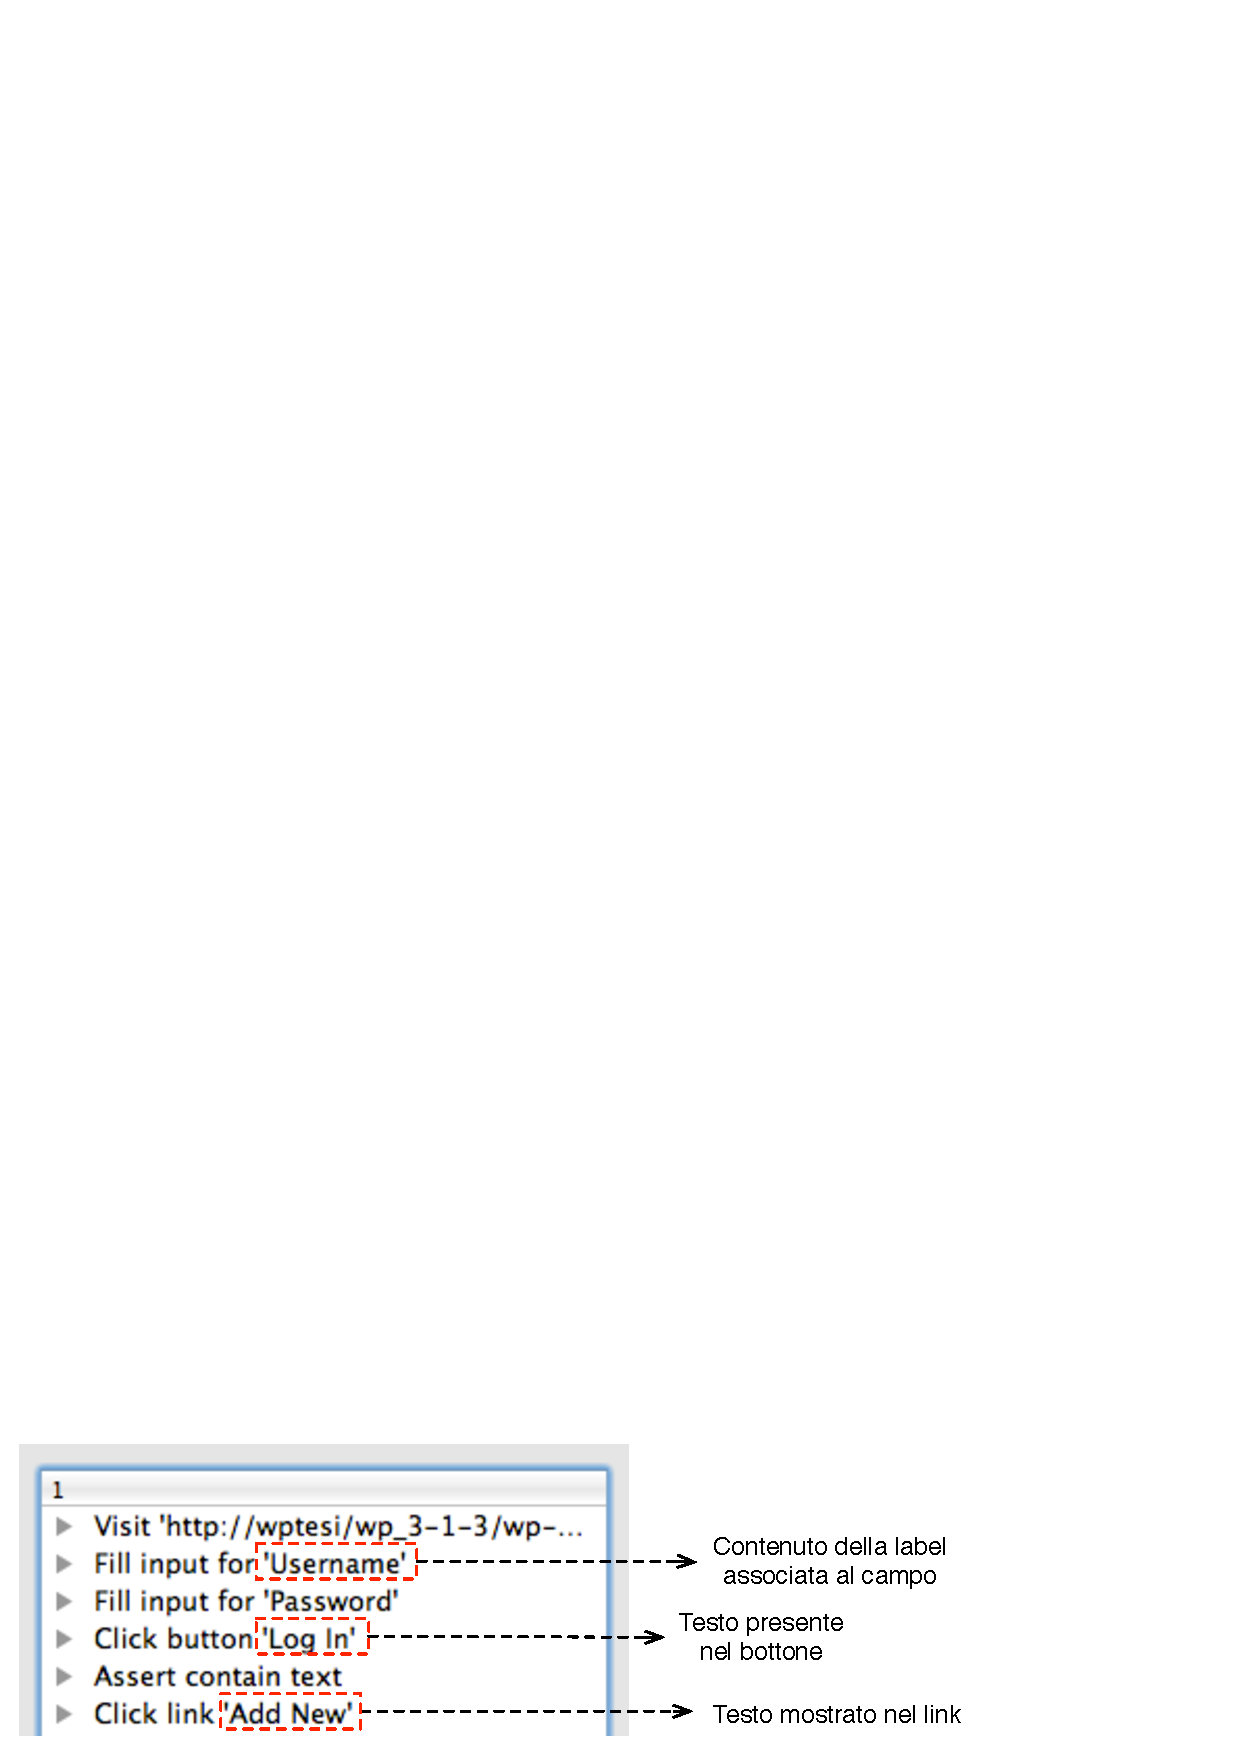
\includegraphics[width=\textwidth]{images/action_notes.png}
\caption{Lista delle azioni registrate mostrata all'utente nell'interfaccia grafica}
\label{fig:actionNotes}
\end{center}
\end{figure}

Si è rivelata di notevole interesse inoltre la funzione \verb|jQuery.live|, qualora l'applicazione web su cui si stanno effettuando i test faccia uso di richieste AJAX. In questi casi è frequente che il DOM venga modificato una volta terminata la richiesta, ad esempio creando nuovi nodi per mostrare nella pagina i dati ricevuti dal server. 

Siccome questi nuovi elementi non erano presenti nel DOM nel momento in cui è stato iniettato il codice Javascript, gli event listener per questi nodi non sono stati registrati e risulterebbe impossibile intercettare gli eventi che li interessano. 

Utilizzando la funzione \verb|jQuery.live| invece che \verb|jQuery.bind|, viene registrato un event listener speciale per il nodo radice dell'albero DOM. Quando l'evento si verifica esso viene propagato dal basso verso l'alto durante la fase di "event bubbling" e poiché non sono associati event listener al nodo del DOM appena inserito, esso raggiunge il nodo radice, dove viene intercettato dall'event listener registrato tramite \verb|.live|. A questo punto viene verificato che l'elemento target coincida con quello specificato per \verb|live| e in caso positivo si procede all'esecuzione del codice di gestione dell'evento. Siccome quest'ultimo passaggio non viene effettuato fino a che l'evento non si verifica, gli elementi che corrispondono al selettore indicato rispondono comunque all'evento, nonostante siano stati aggiunti al DOM in un secondo momento.

Uno scenario tipico viene rappresentato in figura ~\ref{fig:liveEventCase}, dove è necessario poter continuare il test dell'applicazione cliccando su link aggiunto alla pagina dopo la richiesta asincrona.

\begin{figure}[htbp]
\begin{center}
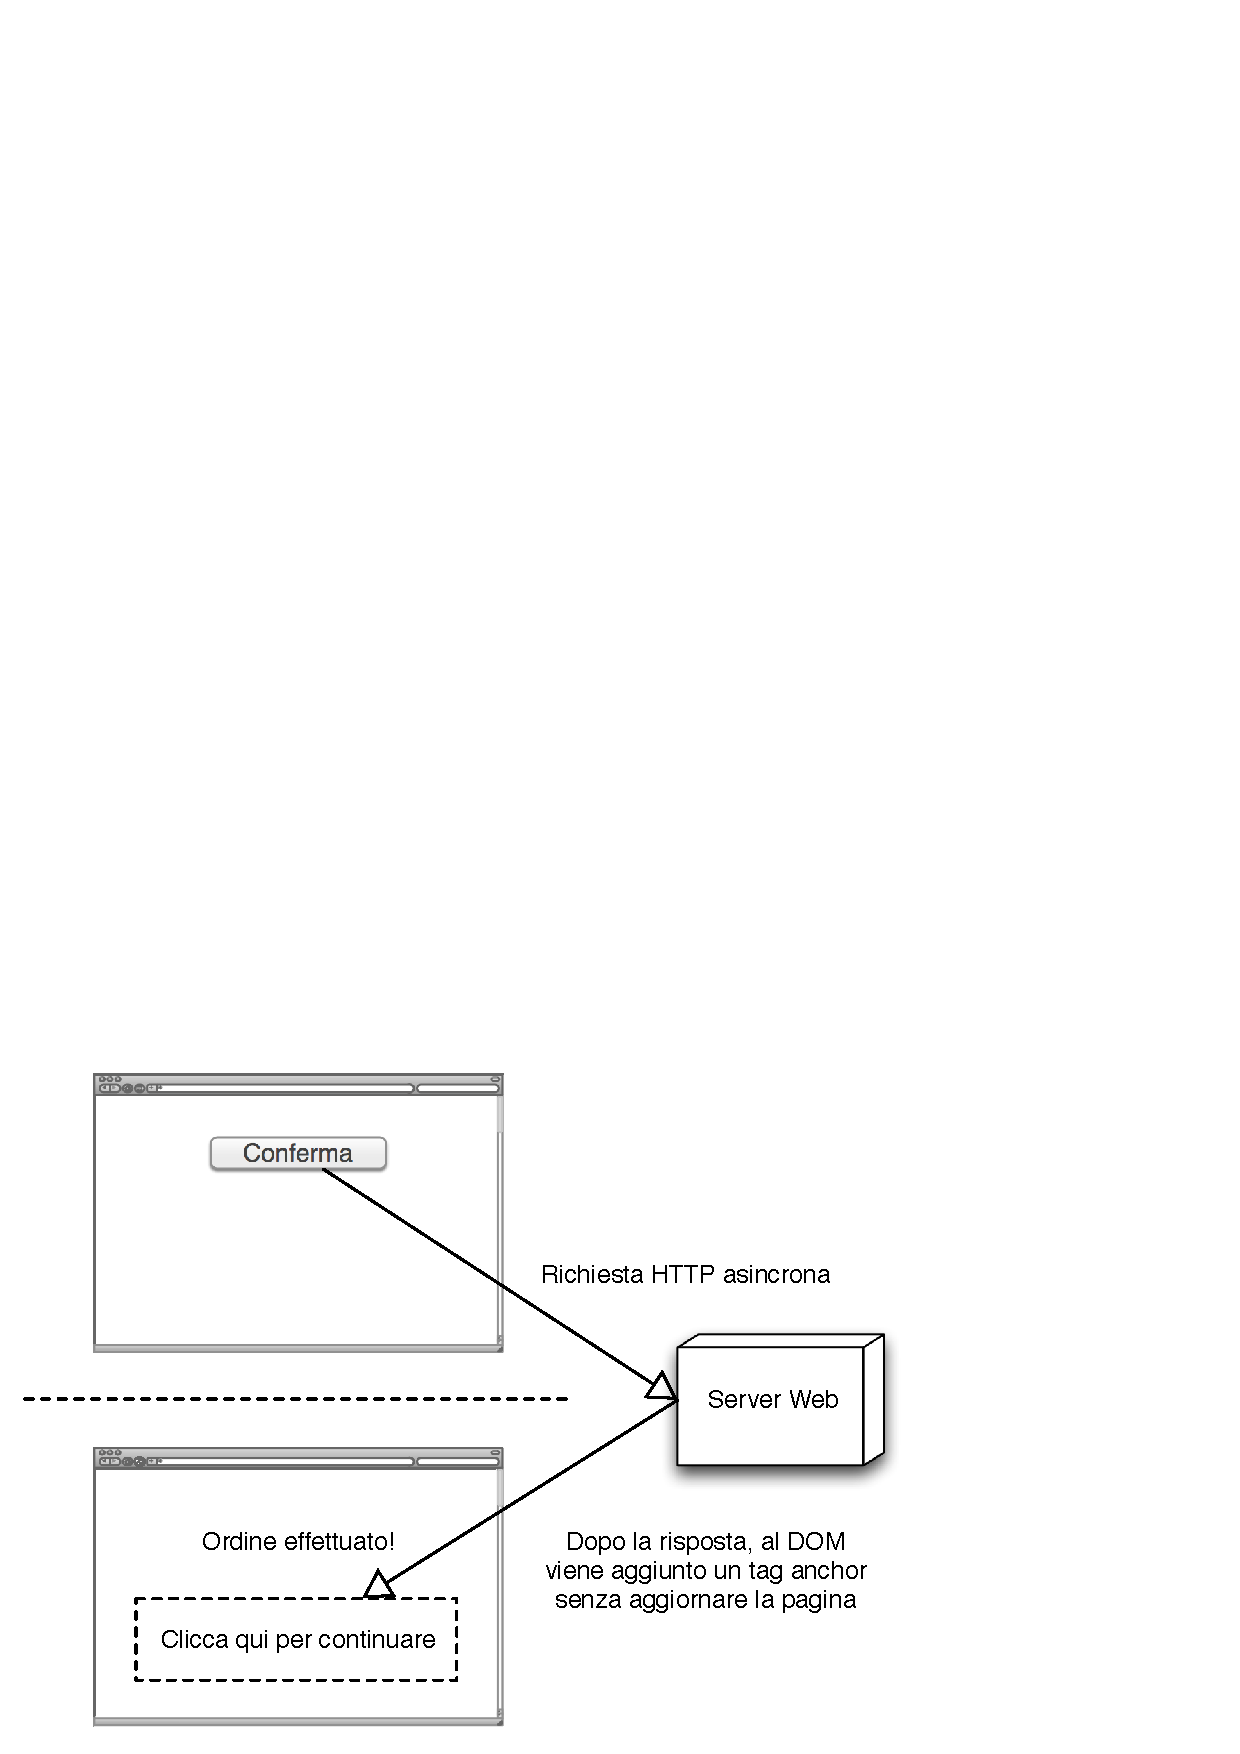
\includegraphics[width=\textwidth]{images/live_event_case.png}
\caption{Esempio di scenario che contempla la modifica del DOM}
\label{fig:liveEventCase}
\end{center}
\end{figure}

%TODO: solo alcuni eventi sono registrati, spiegare ?

\subsection{Riproduzione degli eventi}

Una volta che le azioni compiute dall'utente sulla pagina web sono state registrate mediante la strategia descritta nel paragrafo precedente, è necessario poterle riprodurre in maniera programmatica per simulare l'interazione dell'utente durante la simulazione del test.

Per sintetizzare gli eventi sono state considerate ed implementate due strategie alternative, che verranno ora analizzate nel dettaglio.

\subsubsection{Eventi Javascript}

La soluzione che si è rivelata più semplice consiste nel riprodurre gli eventi tramite codice Javascript, in maniera simmetrica a come essi vengono registrati. Per la scrittura del codice apposito si è tratta in parte ispirazione dal framework YUI Library, rilasciata da Yahoo con licenza BSD, la quale contiene un modulo per la simulazione degli eventi. 

Come punto di partenza si è utilizzata l'API definita dalla specifica DOM Event del W3C, la quale definisce i metodi \verb|createEvent| e \verb|dispatchEvent| per creare un evento di un dato tipo e per avviare la sua propagazione del DOM. Attraverso questi metodi è perciò possibile sintetizzare tutte le tipologie di eventi definite nella specifica, personalizzandone se necessario le proprietà.

Il codice Javascript che si occupa di generare gli eventi è stato implementato come un plugin per la libreria jQuery all'interno del file \verb|jquery.simulate.js| così da integrarne l'utilizzo con l'interfaccia fluente di jQuery. Grazie all'architettura dei plugin, i metodi definiti per creare gli eventi sono invocabili direttamente su di una collezione di nodi del DOM selezionata tramite la sintassi standard di jQuery.

\lstinputlisting[float=h, language=Javascript, caption={Creazione di un evento del mouse in Javascript}, label=code:jsMouseEvent]{code/actions/create_event.js}

Il plugin per la simulazione degli eventi viene iniettato nella pagina dal simulatore subito dopo il termine del caricamento e classi in Python ne possono richiamare le funzionalità all'interno del rispettivo metodo \verb|execute| utilizzando come intermediario la classe \verb|Simulator|. 

Questo meccanismo di sintesi è stato utilizzato per riprodurre gli eventi legati al mouse, come il click o lo spostamento del puntatore sopra un determinato elemento. L'inserimento di una sequenza di caratteri all'interno di un campo di testo e la sezione di un'opzione da un menù a tendina sono stati invece implementati attraverso il metodo \verb|val()| dell'API jQuery, che imposta il valore del campo di input al parametro passato. Questa scelta ha permesso di semplificare la simulazione di questi eventi, che altrimenti avrebbero dovuto essere realizzati attraverso la combinazione di una serie di eventi. E' infatti possibile riprodurre l'inserimento di una stringa in un campo di testo anche attraverso la propagazione di un evento di tipo \verb|keyPress| per ogni carattere della stringa immessa.

I due principali vantaggi di questo approccio sono dati dalla facilità di creare eventi tramite codice Javascript e dal fatto che durante questa operazione ci si trova già direttamente nel contesto del DOM della pagina. Ciò rende più semplice migliorare l'implementazione adottata interagendo se necessario con gli altri elementi. Inoltre, è possibile avvantaggiarsi direttamente dell'uso di jQuery per la manipolazione semplificata degli eventi.

Di contro, lo svantaggio principali risiede nel livello di accuratezza della simulazione che questo metodo fornisce. Quando l'utente effettua un click su di un link di fatto non viene generato un unico evento, bensì si originano una serie di eventi collaterali subito prima e subito dopo l'azione che l'utente ha intenzione di compiere. Nel caso dell'esempio corrente, lo spostamento del mouse sull'elemento \verb|anchor| ne scatena prima di tutto l'evento \verb|onmouseover|. Ancora prima del click vero e proprio, a seconda del tipo l'elemento può ottenere lo stato di focus, che provoca l'omonimo evento.

Nel caso di applicazioni più complesse, a questi eventi collaterali vengono associati degli event listener per implementare alcune funzionalità importanti, come nel caso dell'autocompletamento per un campo di input. A seconda di come sono stati implementati questi dettagli, potrebbe quindi non essere sufficiente simulare un solo evento per riprodurre in maniera verosimile il reale comportamento dell'utente. Tuttavia, nei casi di studio esaminati questo problema non si è mai presentato in maniera tale da compromettere l'esecuzione dei test.

\subsubsection{Eventi nativi}

La seconda strategia analizzata per la simulazione degli eventi nell'applicazione web si avvantaggia degli eventi nativi. 

E' opportuno ricordare che anche l'applicazione realizzata all'interno del framework Qt implementa una gestione interna degli eventi, concettualmente simile a quella presentata per il DOM. Il componente grafico QWebView, che disegna sullo schermo la pagina web caricata, è soggetto come ogni altro widget al meccanismo di propagazione degli eventi. Pertanto quando l'utente effettua un click sul widget QWebView l'evento viene intercettato e quest'ultimo innesca poi la creazione del relativo evento nel DOM della pagina. 

Anziché sintetizzare l'evento di interesse direttamente nel contesto del DOM, si è quindi pensato di sfruttare il controllo esercitabile sull'ambiente esterno per spostare la simulazione dell'evento ad un livello decisamente più basso, molto più vicino a quello del sistema operativo sottostante. 

In questo modo la simulazione è decisamente più accurata, poiché il componente \verb|QWebView| riceve degli eventi del tutto analoghi a quelli che riceverebbe dal loop principale dell'applicazione, provenienti dal sistema operativo, e li riporta in maniera nativa nel contesto della pagina web. Dal punto di vista di quest'ultima non è pertanto possibile distinguere tra un evento reale ed uno simulato attraverso tale strategia in maniera pratica. In figura ~\ref{fig:nativeEvents} è riportato lo schema a blocchi dei componenti interessati durante la simulazione nativa degli eventi.

\begin{figure}[htbp]
\begin{center}
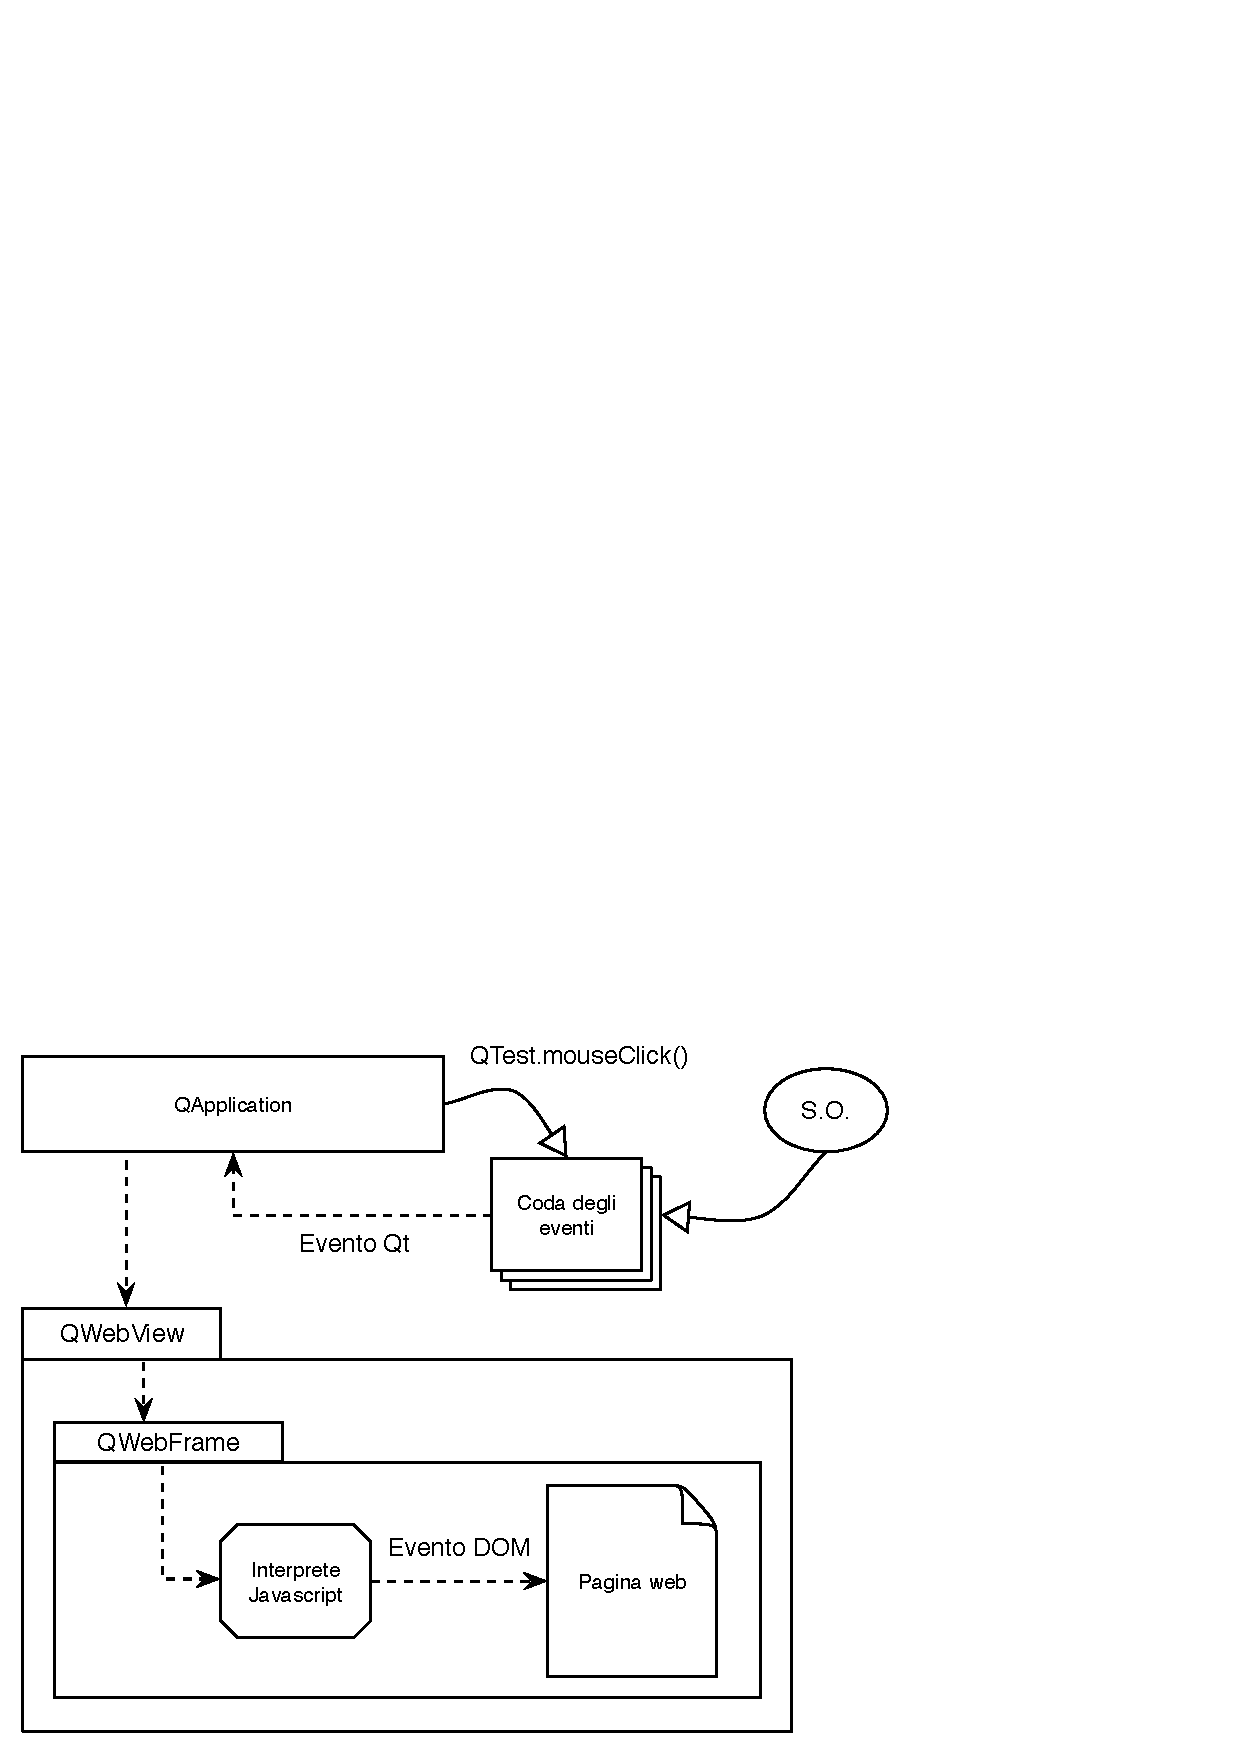
\includegraphics[width=\textwidth]{images/native_events.png}
\caption{Flusso degli eventi per la simulazione nativa}
\label{fig:nativeEvents}
\end{center}
\end{figure}

Per inviare all'applicazione eventi definiti dal framework Qt si possono utilizzare i metodi \verb|QCoreApplication::sendEvent| e \verb|QCoreApplication::postEvent|, che, con alcune differenze interne, inseriscono un oggetto di tipo \verb|QtEvent| nella coda degli eventi dell'applicazione, specificando quale widget deve risultare come primo destinatario di tale evento. L'utilizzo di tali metodi, tentato come primo approccio, ha comportato una serie di problematiche non banali che hanno quindi portato alla ricerca di una soluzione alternativa.

L'attenzione si è quindi spostata sul modulo \verb|QTest| del framework, concepito per facilitare l'esecuzione di test sulle interfacce grafiche realizzate con Qt. Per questo scopo sono presenti alcuni metodi per la simulazione degli eventi, che hanno consentito di aggirare agevolmente gli ostacoli incontrati durante il primo approccio al problema.

Nello specifico sono stati utilizzati principalmente i metodi \verb|QTest:.mouseMove| e \verb|QTest:.mouseClick| per simulare le interazioni principali con il componente \verb|QWebView|, come mostrato nel listato ~\ref{code:nativeClickLink}. In questo estratto si può osservare come l'azione di click su di un link venga riprodotta simulando prima lo spostamento del mouse sul nodo del DOM e poi l'effettiva pressione del tasto sinistro del mouse.

\lstinputlisting[float=h, language=Python, caption={Implementazione nativa dell'azione ClickLink}, label=code:nativeClickLink]{code/actions/click_link_native.py}

Come primo parametro viene indicata l'istanza di classe \verb|QWidget| a cui deve essere recapitata per prima la notifica dell'evento. L'altro parametro comune rappresenta invece le coordinate dello schermo alle quali si deve verificare l'evento simulato, indicate tramite un oggetto di classe \verb|QPoint|.

Per ricavare le coordinate del nodo del DOM destinatario dell'evento si è seguito il seguente approccio. Il simulatore esegue del codice Javascript che richiama il metodo \verb|jQuery.offset| sul nodo selezionato, il quale restituisce l'ascissa e l'ordinata dell'elemento in base alla distanza dal margine sinistro e da quello superiore della pagina. Successivamente viene istanziato un oggetto di classe \verb|QPoint| con i valori ottenuti. 

A questo punto è necessario convertire le coordinate dell'elemento relative al componente \verb|QWebView| al sistema sistema di riferimento della finestra applicativa, in modo da identificare correttamente la posizione utilizzata per simulare l'evento. 

\lstinputlisting[float=h, language=Python, caption={Coordinate del nodo DOM interessato dalla simulazione}, label=code:elementPosition]{code/actions/element_position.py}